\documentclass[a4paper,12pt]{article}

\usepackage[slovene]{babel}
\usepackage[utf8]{inputenc}
\usepackage[T1]{fontenc}
\usepackage{lmodern}
\usepackage{amsmath}
\usepackage{amssymb}
\usepackage{amsthm}
\usepackage{amsfonts}
\usepackage{mathtools}
\usepackage{enumitem}



\begin{document}


%%% naslovna stran

\begin{titlepage}
    \centering
    \vfill
    \vfill
    \textbf{\Huge{Poročilo projekta}}
    \vfill
    \textbf{\LARGE{Matematično modeliranje}}
    \vfill\vfill\vfill\vfill\vfill
    \textsc{\Large{Sara Bizjak}}
    \vfill\vfill
    \textsc{\large{Univerza v Ljubljani}}
    
    \textsc{\large{Fakulteta za matematiko in fiziko}}
    
    \textsc{\large{Oddelek za matematiko}}
    \vfill\vfill
        
    \large{avgust 2019}
    
    \end{titlepage}

\newpage

\tableofcontents

\newpage

\section{\textsc{\large{PREDSTAVITEV PROBLEMA}}}

Rešujemo problem otroka, ki se sprehaja po ravnem igrišču na mivki, za seboj pa vleče na 
vrvico privezano igračo tako, da je vrvica vseskozi napeta. Otrokovo gibanje opišemo s 
parametrično krivuljo. Program izračuna sled gibanja igrače po mivki in izriše animacijo.
\\

\section{\textsc{\large{MATEMATIČNO OZADJE}}}

Rešujemo primer naloge, kjer gibanje igrače določimo z rešitvijo diferencialne enačbe. \\
Ker lahko za rešitev diferencialne enačbe v Matlabu uporabimo že vgrajeno funkcijo {\texttt{ode45}}, bomo reševanje diferencialnih enačb izpustili. 
Ponovimo samo nekaj osnovnih pojmov.
\\
Ker imamo podatek o hitrosti, rešujemo DE prvega reda.
\\
\\
Enačbi, v kateri nastopa neznana funkcija in njen odvod, pravimo \textbf{diferencialna enačba prvega reda}. 
Najsplošnejša oblika diferencialne enačbe prvega reda je
\begin{displaymath}
F(x, y, dy) = 0,
\end{displaymath}
kjer je \textit{F} dana funkcija treh spremenljivk, $y = y(x)$ pa je neznana funkcija.
Smiselno je zahtevati, da je definicijsko območje neznane funkcije odprt interval,
sicer imamo težave z računanjem njenih odvodov.
Pogosto lahko iz $F(x, y, dy) = 0$ izrazimo $dy$ kot funkcijo $x$ in $y$. V tem primeru pravimo,
da smo diferencialno enačbo prevedli na \textbf{standardno obliko}.
\\
\\
Vgrajena Matlabova funkcija za reševanje diferencialnih enačb izgleda takole:
\begin{displaymath}
[X, Y] = ode45(odefun, [x0, b], y0).
\end{displaymath}

\newpage
\section{\textsc{\large{REŠITEV PROBLEMA}}}

Poznamo parametrizacijo krivulje, po kateri se premika otrok. Ker je vrvica med otrokom in 
igračo vedno napeta, vemo, da sta vedno enako oddaljena. Igrača se vedno giba v smeri otroka. 
Poznamo smer igrače, velikost hitrosti pa je odvisna od kota med smerjo gibanja otroka in smerjo vrvice.
Njene pozicije oz. krivuljo gibanja torej dobimo kot rešitev diferencialne enačbe.
\\
\\
Z $x(t)$ in $y(y)$ je označena parametrizacija otroka, z $x_i(t)$ in $y_i(t)$ pa igrače. Odvodi so označeni kot $dx(t), \ dy(t), \ dx_i(t)$ in $dy_i(t)$. \\
Poznamo parametrizacijo otroka, torej $x(t)$ in $y(t)$. Vemo, da vektor hitrosti igrače kaže v smeri proti otroku (po vrvici).
Torej velja

\begin{align*}
    dx_i(t) = x(t) - x_i(t) \\
    dy_i(t) = y(t) - y_i(t). \\
\end{align*}
Vektor smeri normiramo in ga pomnožimo z normo hitrosti otroka.
\\
\begin{align}
     \Big(
    \begin{bmatrix} 
        x(t) \\
        y(t)
    \end{bmatrix}
    -
    \begin{bmatrix} 
        x_i(t) \\
        y_i(t) 
    \end{bmatrix}
    \Big)
    \ \cdot \
    \frac{
    \Big \|
    \begin{bmatrix} 
        dx(t) \\
        dy(t)
    \end{bmatrix}
    \Big \|
    }
    {
    \Big \|
    \begin{bmatrix} 
        x(t) \\
        y(t)
    \end{bmatrix}
    -
    \begin{bmatrix} 
        x_i(t) \\
        y_i(t) 
    \end{bmatrix}
    \Big \|
    }
\end{align}
\\
\\
Da ohranjamo razdaljo oz. napeto vrvico med otrokom in igračo, račun (1) pomnožimo še 
s kotom med hitrostjo otroka in daljico, ki povezuje igračo in otroka. 
Velikost kota dobimo s skalarnim produktom, in sicer

\begin{align}
    \varphi = 
    \frac{
    \begin{bmatrix} 
        dx(t), \ %
        dy(t)
    \end{bmatrix}
    \cdot
    \begin{bmatrix} 
        x(t) - x_i(t) \\
        y(t) - y_i(t)
    \end{bmatrix}
    }
    {
    \Big \|
    \begin{bmatrix} 
        dx(t) \\
        dy(t)
    \end{bmatrix}
    \Big \| 
    \cdot
    \Big \|
    \begin{bmatrix} 
        x(t) - x_i(t) \\
        y(t) - y_i(t)
    \end{bmatrix}
    \Big \| 
    }
    .
\end{align}
\\
\\
Če pomnožimo (1) in (2), dobimo sistem \\
\begin{align}
    \begin{bmatrix} 
        dx_i(t) \\
        dy_i(t) 
    \end{bmatrix}
    =
    \frac{
    \begin{bmatrix} 
        x(t) - x_i(t) \\
        y(t) - y_i(t)
    \end{bmatrix}
    \cdot
    \Big(
    \begin{bmatrix} 
        dx(t), \ %
        dy(t)
    \end{bmatrix}
    \cdot
    \begin{bmatrix} 
        x(t) - x_i(t) \\
        y(t) - y_i(t)
    \end{bmatrix}
    \Big)
    }
    {
    \Big \|
    \begin{bmatrix} 
        x(t) - x_i(t) \\
        y(t) - y_i(t)
    \end{bmatrix}
    \Big \| ^ {2}
    }
    .
\end{align}
\\
\\
Sistem (3) sovpada s funkcijo, ki jo vstavimo v Matlabovo vgrajeno funkcijo za reševanje diferencialnih enačb 
{\texttt{ode45}}.
\\
\\
\begin{align*}
    odefun = @(t,\ P) 
    \
    \frac{
        \begin{bmatrix} 
            x(t) - x_i(t) \\
            y(t) - y_i(t)
        \end{bmatrix}
        \cdot
        \Big(
        \begin{bmatrix} 
            dx(t), \ %
            dy(t)
        \end{bmatrix}
        \cdot
        \begin{bmatrix} 
            x(t) - x_i(t) \\
            y(t) - y_i(t)
        \end{bmatrix}
        \Big)
        }
        {
        \Big \|
        \begin{bmatrix} 
            x(t) - x_i(t) \\
            y(t) - y_i(t)
        \end{bmatrix}
        \Big \| ^ {2}
        },
\end{align*}

\begin{align*}
    kjer \ P = 
        \begin{bmatrix} 
            x_i(t) \\
            y_i(t)
        \end{bmatrix}
    .
    \\
\end{align*}
Pri reševanju je predpostavljeno, da je vrvica dolga toliko, kot je začetna oddaljenost igrače in otroka. 
Igrača svoje gibanje vedno začne v koordinatnem izhodišču, torej v točki (0, 0), kar je tudi nastavljen začetni pogoj pri reševanju diferencialne enačbe. 


\subsection{\textsc{Matlabove datoteke}}

Rešitev diferencialne enačbe izračunamo s funkcijo v datoteki {\texttt{igraca.m}}. Datoteki {\texttt{risi\_otrok.m}} in {\texttt{risi\_igraca.m}} izriseta krivuljo, 
po kateri se gibata otrok oziroma igrača. Gibanje izrišemo s pomočjo {\texttt{animacija.m}}. 
Vse skupaj poženemo z datoteko {\texttt{test.m}}, kjer sta določena parametrizacija krivulje, po kateri se giba otrok, in njen odvod.

\newpage
\section{\textsc{\large{PRIMERI GIBANJA}}}

Poglejmo si nekaj primerov gibanja. Modra barva krivulje označuje gibanje otroka, rdeča pa igrače.

\subsection{\textsc{Primer 1}}
    
     Gibanje otroka po krivulji s parametrizacijo:
    \begin{center}
    $x(t) = cos(t)$, \\
    $y(t) = sin(t)$. 
    \end{center}
    Če se otrok premika v krogu, igrača pa je na začetku v središču kroga (torej je vrvica dolga enako kot radij - predpostavka), ostane igrača ves čas na istem mestu.
    \\
    \\
    \begin{figure}[!h]
        \centering
        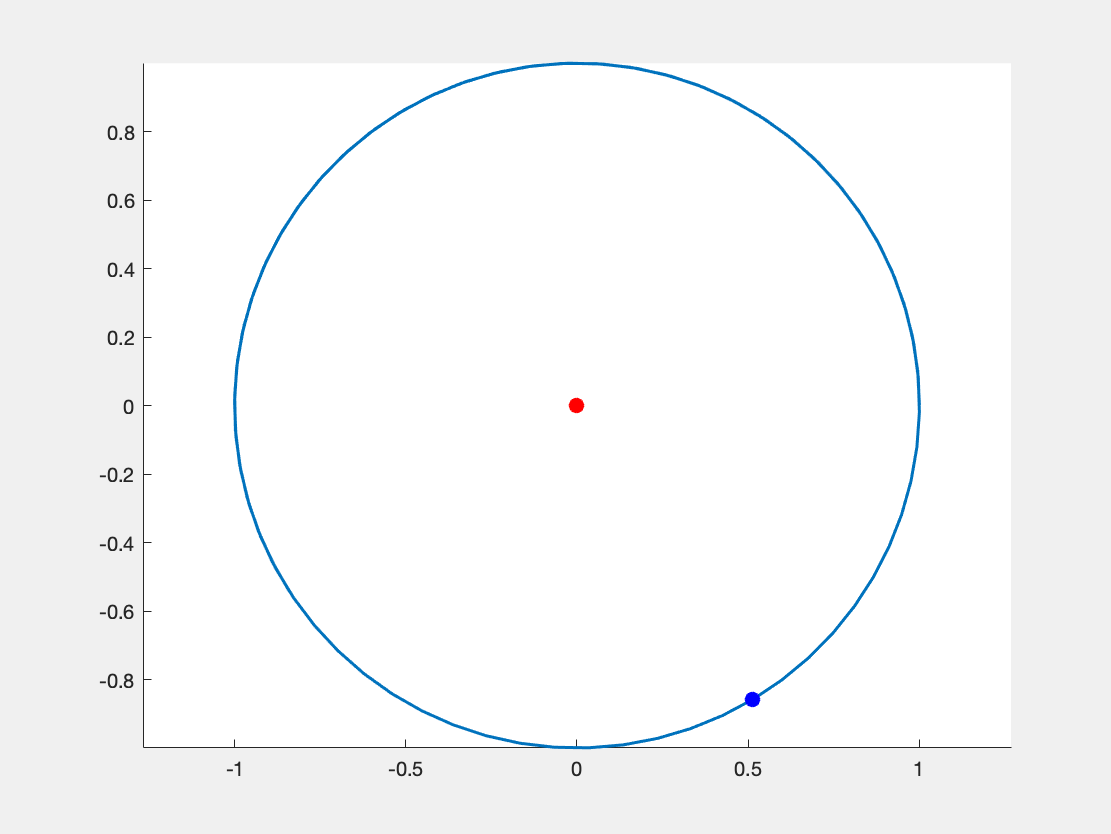
\includegraphics[scale=0.4]{Primer1}
    \end{figure}

    \newpage
   
    \subsection{\textsc{Primer 2}}
     Gibanje otroka po krivulji s parametrizacijo:
    \begin{center}
    $x(t) = t + cos(t)$, \\
    $y(t) = t + sin(t)$. 
    \end{center}      
    \begin{figure}[!h]
        \centering
        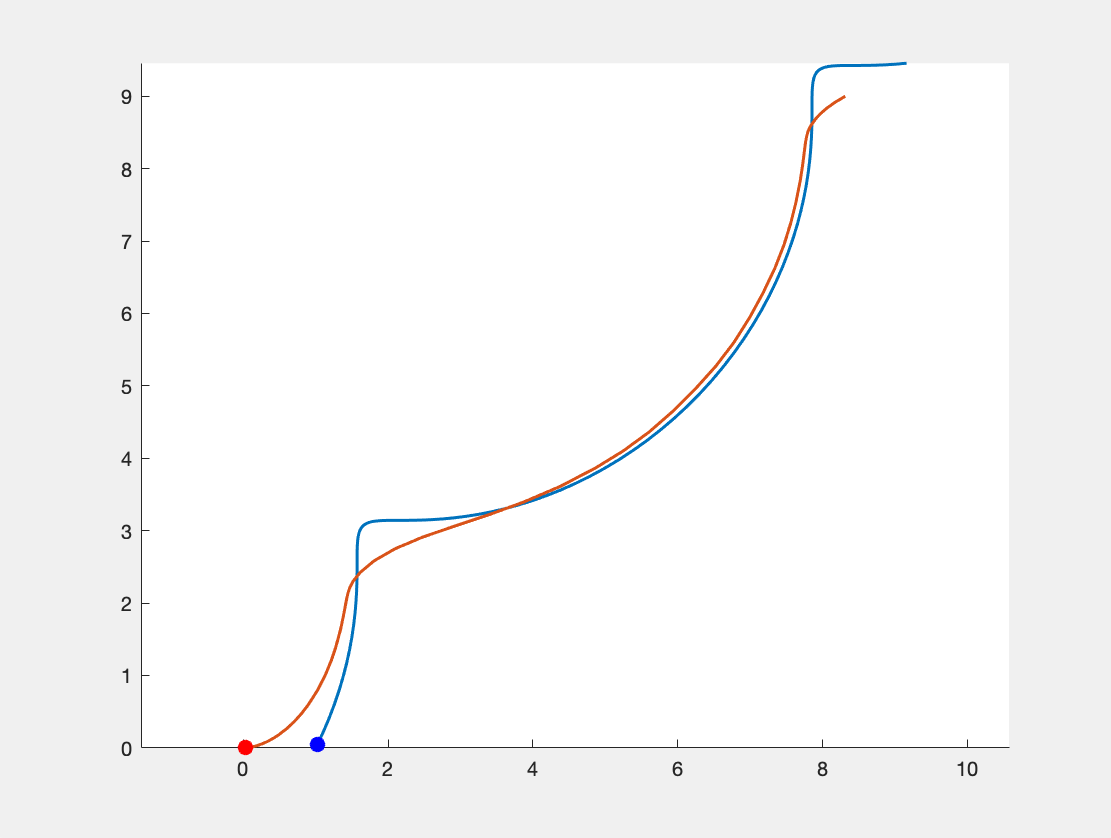
\includegraphics[scale=0.4]{Primer2}
    \end{figure}

    \subsection{\textsc{Primer 3}}
    Gibanje otroka po krivulji s parametrizacijo:
    \begin{center}
    $x(t) = t + cos(t)$, \\
    $y(t) = t - sin(t)$. 
    \end{center}      
    \begin{figure}[!h]
        \centering
        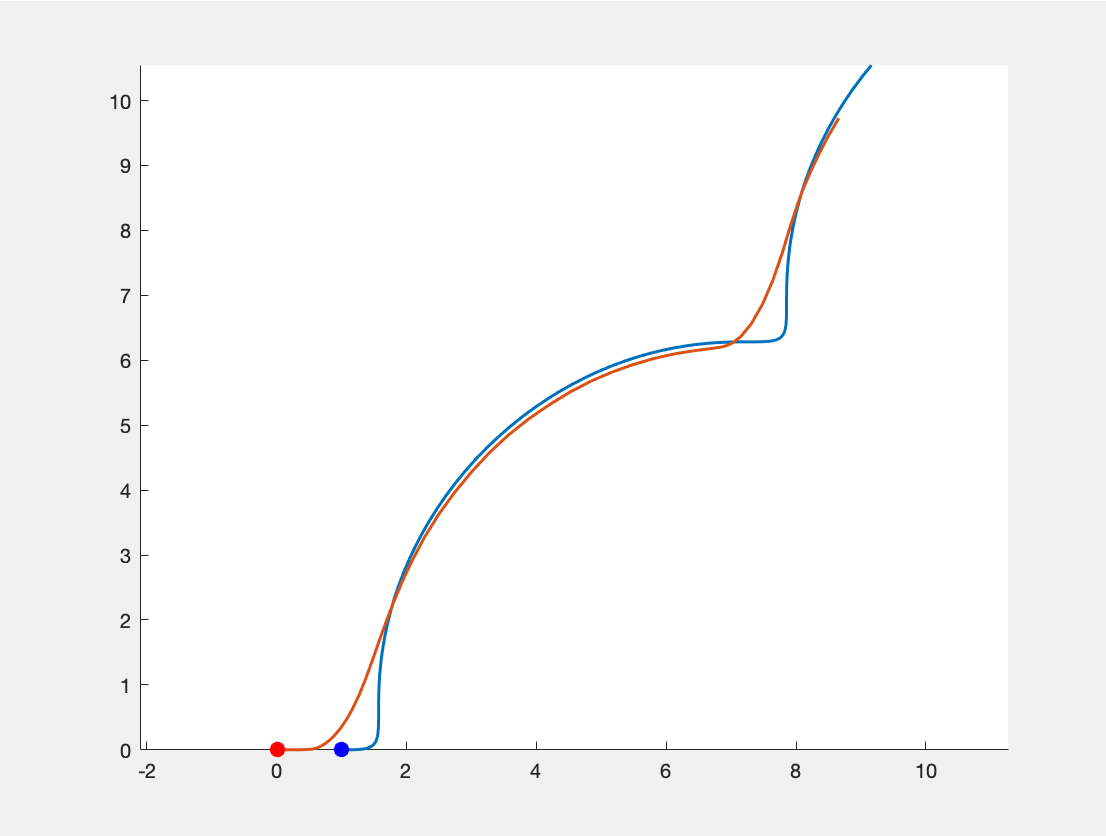
\includegraphics[scale=0.4]{Primer3}
    \end{figure}
    
    \newpage
    \subsection{\textsc{Primer 4}}
    Gibanje otroka po krivulji s parametrizacijo:
    \begin{center}
    $x(t) = t + cos(t) + sin(t)$, \\
    $y(t) = t + sin(t) - cos(t)$. 
    \end{center}      
    \begin{figure}[!h]
        \centering
        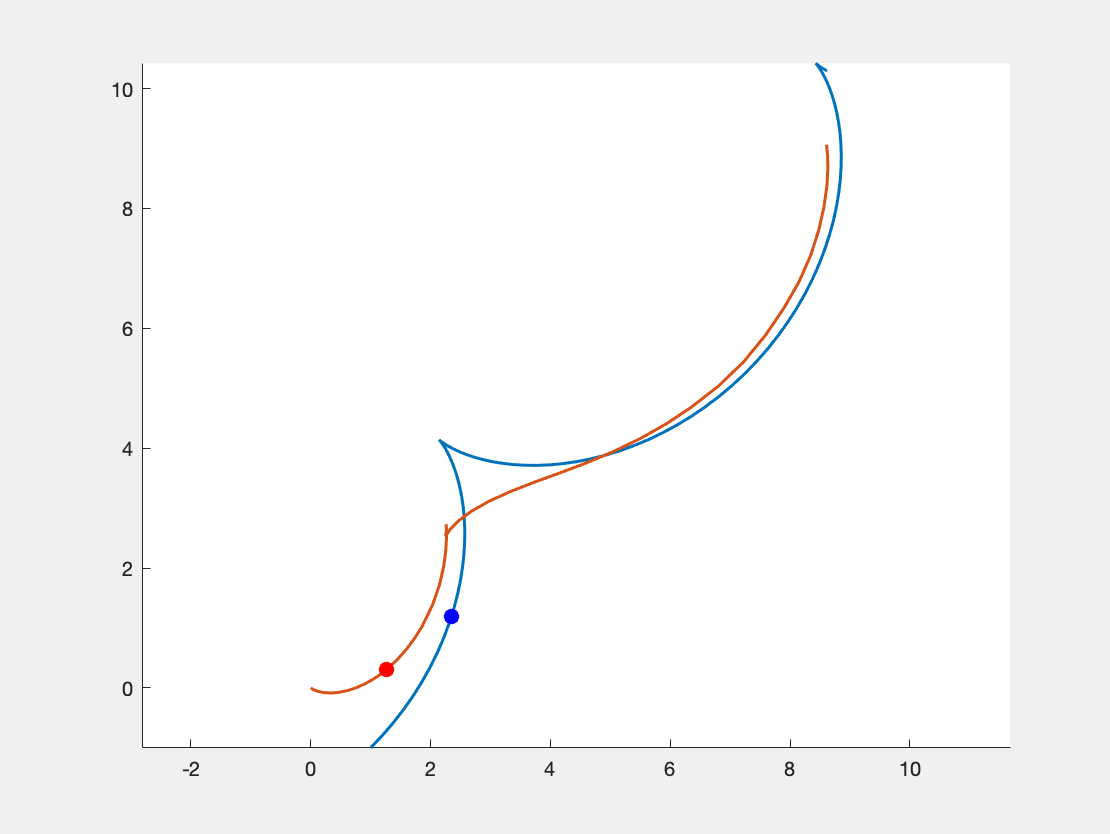
\includegraphics[scale=0.4]{Primer4}
    \end{figure}
    
    \subsection{\textsc{Primer 5}}
    Gibanje otroka po krivulji s parametrizacijo:
    \begin{center}
    $x(t) = t + cos(t) - sin(t)$, \\
    $y(t) = t + sin(t) + cos(t)$. 
    \end{center}      
    \begin{figure}[!h]
        \centering
        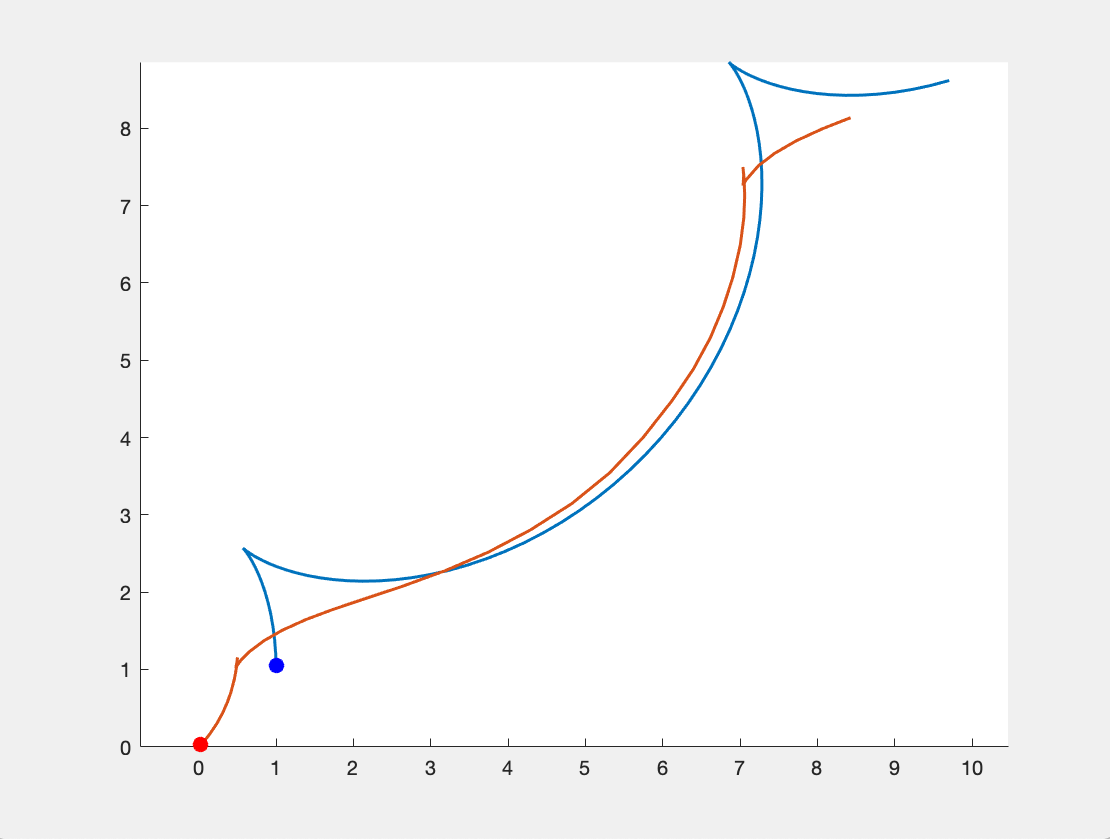
\includegraphics[scale=0.4]{Primer5}
    \end{figure}

\newpage

\section{\textsc{\large{ZAKLJUČEK}}}


\newpage	
\begin{thebibliography}{99}
	\bibitem{a} 
	J Cimprič: Diferencialne enačbe, FMF, skripta, dostopno na https://www.fmf.uni-lj.si/~cimpric/skripta/del6.pdf.

\end{thebibliography}

\end{document}